\documentclass{beamer}
%%%%%%%%%%%%%%%%%%%%%%%%%%%%%%%%%%%%%%%%%%%%%%%%%%%%%%%%%%%%%%%%%%%%%%%%%%%%%%%%%%%%%%%%%%%%%%%%%%
\setbeamertemplate{navigation symbols}{}
\usepackage{beamerthemeshadow}
\usefonttheme{serif}
%%%%%%%%%%%%%%%%%%%%%%%%%%%%%%%%%%%%%%%%%%%%%%%%%%%%%%%%%%%%%%%%%%%%%%%%%%%%%%%%%%%%%%%%%%%%%%%%%%
\usepackage{graphicx}
\graphicspath{ {res/} }
%%%%%%%%%%%%%%%%%%%%%%%%%%%%%%%%%%%%%%%%%%%%%%%%%%%%%%%%%%%%%%%%%%%%%%%%%%%%%%%%%%%%%%%%%%%%%%%%%%
\usepackage{polyglossia}
\setdefaultlanguage{armenian}
\setotherlanguages{english}
\usepackage{fontspec}
\newfontfamily\armenianfont{DejaVu Sans}
%%%%%%%%%%%%%%%%%%%%%%%%%%%%%%%%%%%%%%%%%%%%%%%%%%%%%%%%%%%%%%%%%%%%%%%%%%%%%%%%%%%%%%%%%%%%%%%%%%
\usepackage{minted}
\setminted[cpp]{fontsize=\footnotesize}
\setmonofont{Consolas}
%%%%%%%%%%%%%%%%%%%%%%%%%%%%%%%%%%%%%%%%%%%%%%%%%%%%%%%%%%%%%%%%%%%%%%%%%%%%%%%%%%%%%%%%%%%%%%%%%%
\usepackage{xltxtra}
\usepackage{hyperref}
%%%%%%%%%%%%%%%%%%%%%%%%%%%%%%%%%%%%%%%%%%%%%%%%%%%%%%%%%%%%%%%%%%%%%%%%%%%%%%%%%%%%%%%%%%%%%%%%%%
\usetheme{Luebeck}
\usecolortheme{crane}
%%%%%%%%%%%%%%%%%%%%%%%%%%%%%%%%%%%%%%%%%%%%%%%%%%%%%%%%%%%%%%%%%%%%%%%%%%%%%%%%%%%%%%%%%%%%%%%%%%
\definecolor{HTDark}{rgb}{0.04706, 0.13725, 0.26667} % primary color
\definecolor{HTLight}{rgb}{0.3686, 0.5255, 0.6235}   % secondary color
\setbeamercolor{palette primary}{bg=HTDark,fg=white}
\setbeamercolor{palette secondary}{bg=HTDark,fg=white}
\setbeamercolor{palette tertiary}{bg=HTDark,fg=white}
\setbeamercolor{palette quaternary}{bg=HTDark,fg=white}
\setbeamercolor{structure}{fg=HTDark} % itemize, enumerate, etc
\setbeamercolor{section in toc}{fg=HTDark} % TOC sections
\setbeamercolor{block title}{fg=white,bg=HTDark}
\setbeamercolor{block body}{fg=white, bg=HTLight}
\setbeamercolor{subsection in head/foot}{bg=HTLight,fg=white}
%%%%%%%%%%%%%%%%%%%%%%%%%%%%%%%%%%%%%%%%%%%%%%%%%%%%%%%%%%%%%%%%%%%%%%%%%%%%%%%%%%%%%%%%%%%%%%%%%%


\begin{document}

\title[Proxy]{Նախագծման Ձևանմուշներ։ Proxy}
\author[Հրաչյա Թանդիլյան\copyright]{Հրաչյա Թանդիլյան}
\date{2020}

%-------------------------------------------------------------------------------------------------
\begin{frame}
\titlepage
\end{frame}
%-------------------------------------------------------------------------------------------------

\section{Նպատակը}
%-------------------------------------------------------------------------------------------------
\begin{frame}\frametitle{Proxy}
\begin{block}{Նպատակը}
    Տվյալ օբյեկտի համար տրամադրել այնպիսի փոխարինող, որը կվերահսկի նրան դիմումը:
\end{block}
\vfill
Նաև հայտնի է որպես
\begin{itemize}
    \item Surrogate
\end{itemize}
\end{frame}
%-------------------------------------------------------------------------------------------------

\subsection{Մոտիվացիան}
%-------------------------------------------------------------------------------------------------
\begin{frame}\frametitle{Մոտիվացիան}
\begin{center}
    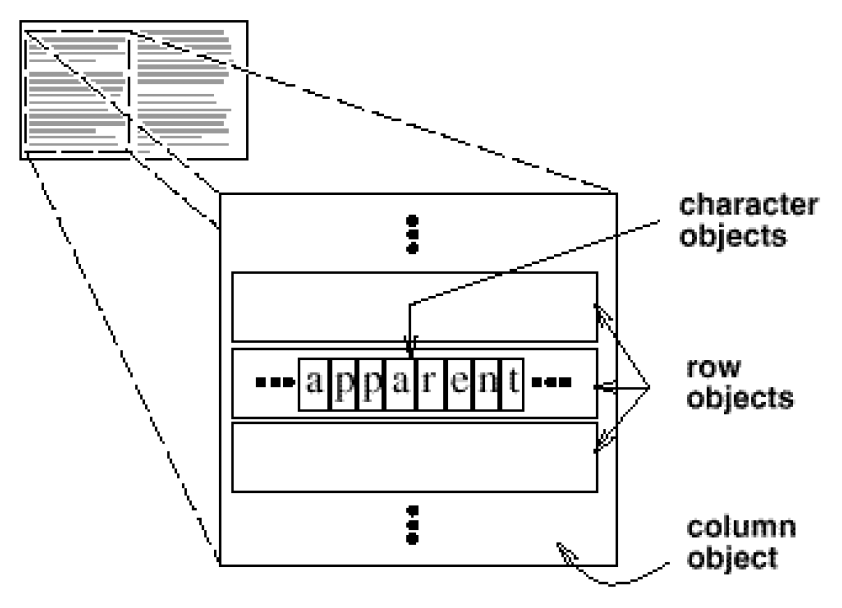
\includegraphics[scale=0.4]{motivation1.png}
\end{center}
\end{frame}
%-------------------------------------------------------------------------------------------------

%-------------------------------------------------------------------------------------------------
\begin{frame}\frametitle{Մոտիվացիան}
\begin{center}
    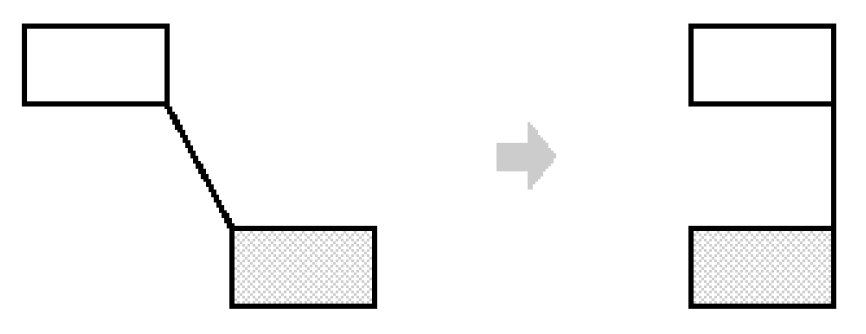
\includegraphics[scale=0.4]{motivation2.png}
\end{center}
\end{frame}
%-------------------------------------------------------------------------------------------------

\subsection{Կիրառելիությունը}
%-------------------------------------------------------------------------------------------------
\begin{frame}\frametitle{Կիրառելիությունը}
Այս Ն.Ձ. պետք է օգտագործել երբ.
\vfill
\begin{enumerate}
    \item Remote Proxy \pause \vfill
    \item Virtual Proxy \pause \vfill
    \item Protection Proxy \pause \vfill
    \item Smart Reference
\end{enumerate}
\end{frame}
%-------------------------------------------------------------------------------------------------

\section{Կառուցվածքը}
%-------------------------------------------------------------------------------------------------
\begin{frame}\frametitle{Կառուցվածքը}
\begin{center}
    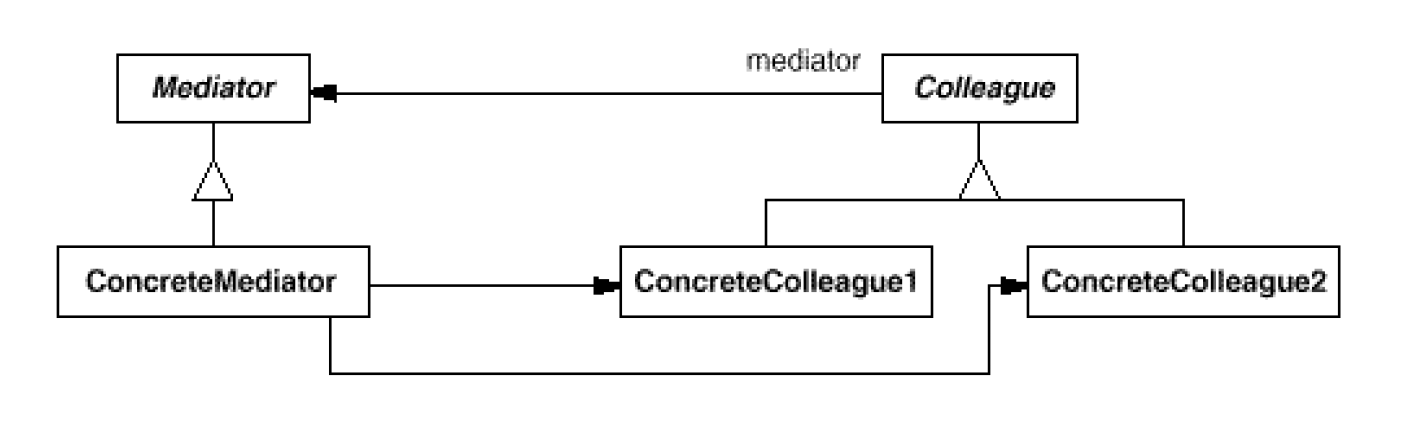
\includegraphics[scale=0.4]{structure1.png}
    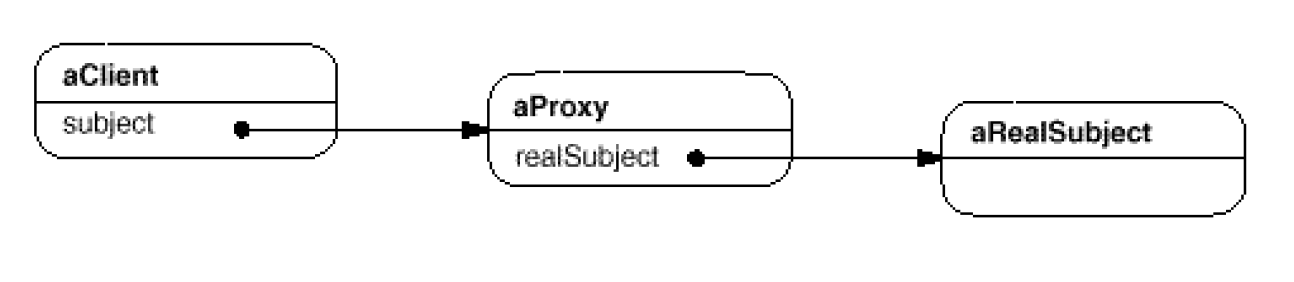
\includegraphics[scale=0.4]{structure2.png}
\end{center}
\end{frame}
%-------------------------------------------------------------------------------------------------

\subsection{Հետևանքները}
%-------------------------------------------------------------------------------------------------
\begin{frame}\frametitle{Հետևանքները}
Այս Ն.Ձ. ունի հետևյալ առավելություններն ու թերությունները.
\vfill
\setbeamertemplate{itemize/enumerate subbody begin}{\scriptsize}
\begin{enumerate}
    \item Վերհղման (indirection) մակարդակ է ավելացնում:
    Կախված Proxy-ի տարատեսակից այդ վերհղումը ունի տարբեր նպատակներ \vfill
    \begin{itemize}
        \item remote proxy-ին թաքցնում է այն փաստը, որ հղվող օբյեկտը գտնվում
        է այլ համակարգչի վրա: \vfill
        \item virtual proxy-ին հնարավորություն է տալիս օբյեկտը ստեղծել
        առաջին դիմման ժամանակ: \vfill
        \item protection proxy-ին և smart reference-ները թույլ են տալիս օբյեկտին
        դիմելիս հավելյալ գործողություններ կատարել: \vfill
    \end{itemize}
    \item copy-on-write օպտիմիզացիաի հնարավորություն է տալիս:
\end{enumerate}
\end{frame}
%-------------------------------------------------------------------------------------------------

\section{Իրականացումը}
%-------------------------------------------------------------------------------------------------
\begin{frame}\frametitle{Իրականացումը}
\begin{enumerate}
    \item Անդամներին դիմման օպերատորի (operator *, operator ->) վերաբեռնում (C++): \vfill
    \item Proxy-ն պարտադիր չէ, որ իմանա իրական օբյեկտի տիպը:
\end{enumerate}
\end{frame}
%-------------------------------------------------------------------------------------------------

\subsection{Օրինակ}
%-------------------------------------------------------------------------------------------------
\begin{frame}[fragile]\frametitle{Օրինակ}
\begin{english}
\begin{minted}{cpp}
class Graphic {

public:
    virtual ~Graphic();
    virtual void Draw(const Point& at) = 0;
    virtual void HandleMouse(Event& event) = 0;
    virtual const Point& GetExtent() = 0;
    virtual void Load(istream& from) = 0;
    virtual void Save(ostream& to) = 0;

protected:
    Graphic();
};
\end{minted}
\end{english}
\end{frame}
%-------------------------------------------------------------------------------------------------

%-------------------------------------------------------------------------------------------------
\begin{frame}[fragile]\frametitle{Օրինակ}
\begin{english}
\begin{minted}{cpp}
class Image : public Graphic {

public:
    Image(const char* file); // loads image from a file
    virtual ~Image();
    virtual void Draw(const Point& at);
    virtual void HandleMouse(Event& event);
    virtual const Point& GetExtent();
    virtual void Load(istream& from);
    virtual void Save(ostream& to);

private:
    // private fields
};
\end{minted}
\end{english}
\end{frame}
%-------------------------------------------------------------------------------------------------

%-------------------------------------------------------------------------------------------------
\begin{frame}[fragile]\frametitle{Օրինակ}
\begin{english}
\begin{minted}[fontsize=\scriptsize]{cpp}
class ImageProxy : public Graphic {

public:
    ImageProxy(const char* imageFile);
    virtual ~ImageProxy();
    virtual void Draw(const Point& at);
    virtual void HandleMouse(Event& event);
    virtual const Point& GetExtent();
    virtual void Load(istream& from);
    virtual void Save(ostream& to);

protected:
    Image* GetImage();

private:
    Image* image;
    Point extent;
    char* fileName;
};
\end{minted}
\end{english}
\end{frame}
%-------------------------------------------------------------------------------------------------

%-------------------------------------------------------------------------------------------------
\begin{frame}[fragile]\frametitle{Օրինակ}
\begin{english}
\begin{minted}[fontsize=\scriptsize]{cpp}
ImageProxy::ImageProxy(const char* f) {
    fileName = strdup(f);
    extent = Point::Zero;
    image = 0;
}

Image* ImageProxy::GetImage() {
    if (image == NULL) {
        image = new Image(fileName);
    }
    return image;
}

const Point& ImageProxy::GetExtent() {
    if (extent == Point::Zero) {
        extent = GetImage()->GetExtent();
    }
    return extent;
}
\end{minted}
\end{english}
\end{frame}
%-------------------------------------------------------------------------------------------------

%-------------------------------------------------------------------------------------------------
\begin{frame}[fragile]\frametitle{Օրինակ}
\begin{english}
\begin{minted}{cpp}
void ImageProxy::Draw(const Point& at) {
    GetImage()->Draw(at);
}

void ImageProxy::HandleMouse(Event& event) {
    GetImage()->HandleMouse(event);
}

void ImageProxy::Save(ostream& to) {
    to << extent << fileName;
}

void ImageProxy::Load(istream& from) {
    from >> extent >> fileName;
}
\end{minted}
\end{english}
\end{frame}
%-------------------------------------------------------------------------------------------------

%-------------------------------------------------------------------------------------------------
\begin{frame}[fragile]\frametitle{Օրինակ}
\begin{english}
\begin{minted}{cpp}
class TextDocument {

public:
    TextDocument();
    void Insert(Graphic*);
    // other methods
};

TextDocument* text = new TextDocument;
text->Insert(new ImageProxy("anImageFileName"));
\end{minted}
\end{english}
\end{frame}
%-------------------------------------------------------------------------------------------------

\section{Առնչվող Ձևանմուշները}
%-------------------------------------------------------------------------------------------------
\begin{frame}\frametitle{Առնչվող Նախագծման Ձևանմուշները}
\begin{itemize}
    \item Adapter \vfill
    \item Decorator
\end{itemize}
\end{frame}
%-------------------------------------------------------------------------------------------------

\end{document}
